\documentclass{article}

% if you need to pass options to natbib, use, e.g.:
% \PassOptionsToPackage{numbers, compress}{natbib}
% before loading nips_2016
%
% to avoid loading the natbib package, add option nonatbib:
% \usepackage[nonatbib]{nips_2016}

\PassOptionsToPackage{numbers,sort&compress}{natbib}
\usepackage[final]{nips_2016} % produce camera-ready copy

\usepackage[utf8]{inputenc} % allow utf-8 input
\usepackage[T1]{fontenc}    % use 8-bit T1 fonts
\usepackage{hyperref}       % hyperlinks
\usepackage{url}            % simple URL typesetting
\usepackage{booktabs}       % professional-quality tables
\usepackage{amsfonts}       % blackboard math symbols
\usepackage{nicefrac}       % compact symbols for 1/2, etc.
\usepackage{microtype}      % microtypography
\usepackage{graphicx}
\usepackage{float}
\usepackage{amsmath}
\usepackage{graphicx}
\usepackage{booktabs}
\usepackage{subcaption}
\title{Hit Song Prediction and Playlist Classification by Listener Mood }

% The \author macro works with any number of authors. There are two
% commands used to separate the names and addresses of multiple
% authors: \And and \AND.
%
% Using \And between authors leaves it to LaTeX to determine where to
% break the lines. Using \AND forces a line break at that point. So,
% if LaTeX puts 3 of 4 authors names on the first line, and the last
% on the second line, try using \AND instead of \And before the third
% author name.

\author{
  Student number\\s2845408
  %% examples of more authors
  \And
  Student number\\s2772327
 \And
  Student number\\s2777346
   \And
  Student number\\s2810265
}

\begin{document}

\maketitle

\begin{abstract}
This report investigates song popularity prediction using and emotion-aware playlist clustering from Spotify dataset. We evaluate multiple preprocessing strategies and classifiers, finding that a Linear SVM achieves the best performance (F1 = 0.430, ROC-AUC = 0.531), and also shows a reasonable generalisation gap compared to XGBoost and Gradient Boosting, which exhibit strong overfitting. We then take this model forward for feature-importance analysis and find insights showing that artist reputation dominates prediction performance, while audio features contribute less. After that, an analysis of K-Means clustering using energy and valence was performed to explore the possibility of separating songs by mood for playlist construction.
\end{abstract}


\end{itemize}




\setcounter{section}{0}
\section{Introduction}
Spotify is one of the global music-streaming platforms used worldwide. Furthermore, the audio features calculated for each song, together with the daily Global Top 200 hits, provide an opportunity for analysis for the artists who create and perform music, as well as for the music-related industry. Predicting popular songs is a useful task that could provide companies with insight for better understanding of what makes a song popular. There are various previous publications that use Spotify audio features to predict popular songs \cite{ref1}  \cite{ref2}  \cite{ref3}. All three of these papers use the Spotify dataset from the Spotify API. The dataset they used already contains a popularity score as the label of a popular song, and they rely on audio features as inputs for prediction. These papers achieved the best results using classification models such as logistic regression, Support Vector Machines, and Random Forests, with CNNs providing the highest F1-score and accuracy in prediction \cite{ref4}. These studies raise the question of how they can claim to predict song popularity solely from audio features. In this report, we will extend the study by exploring artist and temporal features to predict the popularity of a song, to ultimately answer the question of what features drive the popularity of music whether it is the artist or something about the song. Also, the report shows how we can estimate the popularity score from the 200 daily hits, which is a challenge because the data we have do not provide the popularity score from Spotify itself. We will examine optimal preprocessing and appropriate dimensionality reduction to achieve the best performance with a variety of classification methods. Furthermore, we will also look at unsupervised models to suggest suitable playlists based on listener mood defined by two dimensions, valence and energy \cite{ref5}, so that listeners can have a playlist that matches the current stage of their emotion.


\section{Exploratory Data Analysis}
The Spotify dataset is processed to remove duplicated songs by id and check the data quality specifically in audio features and we think it is importance of the features for predict the hit song. By checking the audio feature definition in Spotify API in \hyperref[tab:Audio Feature]{Appendix D}, we found that there are 7 audio features. In our data, all features are scaled in a range between 0 and 1. We also convert loudness unit from dBm and plot all the 7 audio features in Figure 1 (a) as box-plots to see the distribution. Instrumentalness and speechiness show highly right-skewed distributions with the most values concentrated near zero, indicating that chart-topping songs predominantly feature vocals rather than purely instrumental or spoken content. In contrast, energy, danceability, and loudness are concentrated at higher values (0.6-0.8 range), suggesting that popular music tends to be energetic, danceable, and loud. Valence displays more uniform distribution than others, indicating that both positive and negative emotional tones can achieve popularity. Box plot analysis reveals outliers across multiple audio features, most notably instrumentalness and speechiness. Despite their statistical designation as outliers using the IQR method (1.5×IQR), all outliers were retained for model training to preserve the full diversity of chart performing music. These skewed distributions necessary to do feature scaling will be applied during preprocessing to ensure all features contribute equally to model training. 
\vspace{-1em}
\begin{figure}[H]
\centering

\begin{subfigure}{0.48\textwidth}
    \centering
    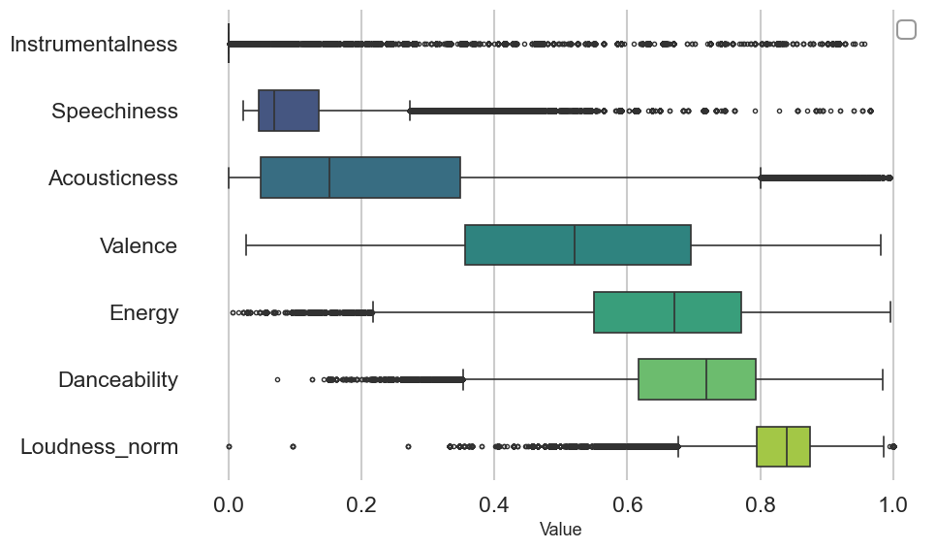
\includegraphics[width=\textwidth]{images/Picture2.png}
    \caption{Distribution of audio features.}
    \label{fig:boxplot}
\end{subfigure}
\begin{subfigure}{0.3\textwidth}
    \centering
    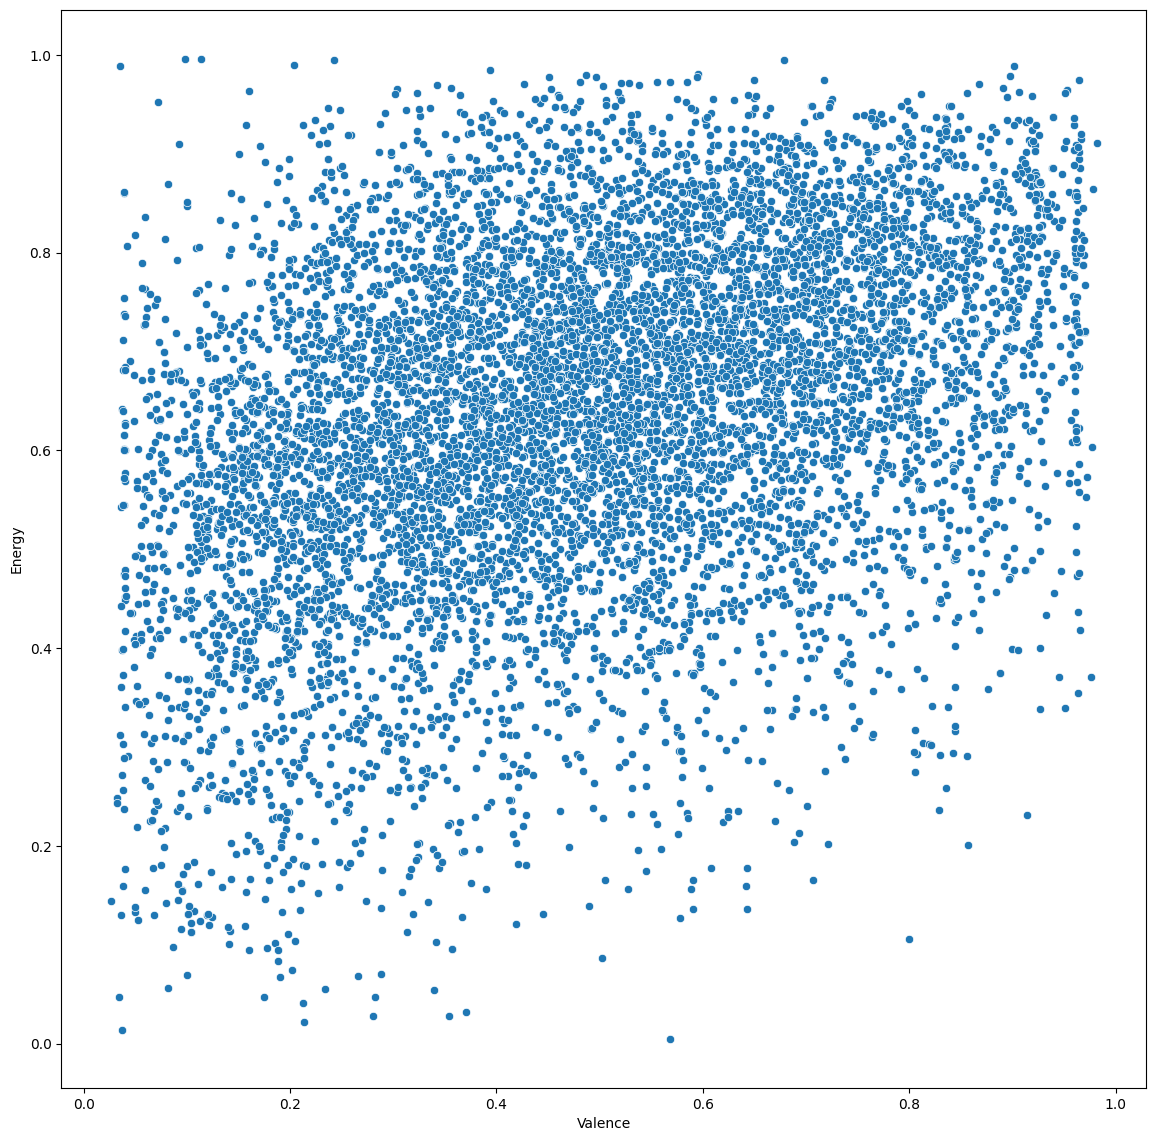
\includegraphics[width=\textwidth]{images/ValenceVSEnergy.png}
    \caption{Valence vs Energy scatter plot.}
    \label{fig:scatter}
\end{subfigure}

\caption{Two visualisations of audio features.}
\label{fig:two_plots}
\end{figure}
\vspace{-2em}
A particularly interesting pattern emerged in the relationship between valence and energy, as illustrated in Figure 1(b). The scatter plot reveals a widely dispersed distribution without a clear linear correlation, suggesting that songs with varying emotional valences (positive to negative) can exhibit any energy level. This broad spread indicates significant diversity in the emotional-energy combinations present in chart-performing music. Further study of these two features revealed their potential utility as song mood classifiers according to the Russell's Circumplex Model of Affect \cite{russell1980circumplex}, which categorizes music into quadrants based on valence (emotional positivity) and energy (arousal level), enabling mood-based classification such as 'happy-energetic', 'calm-peaceful', 'sad-melancholic', and 'angry-tense'. 



We take a look at the artist by plot the distribution of the top 20 artists over the period of data and the distribution song per artist as Figure 2. We can observe that the distribution is right-skewed and a minority of artist are taken into account of the majority of songs in the chart.  Figure 2(b) shows that most artists have only 2 songs on the charts (median), but the average is 6.1 songs per artist. This large difference happens because a few successful artists have many chart hits while most artists have very few. Figure 2(a) shows this clearly Taylor Swift has 211 chart entries, which is over 100 times more than the typical artist. This pattern suggests that famous artists with large fanbases and industry support have an advantage for getting on the charts, regardless of how good each individual song is. Therefore, we create features that track each artist's past chart success (number of previous hits, their typical chart position, and how recently they had a hit) to account for this artist reputation effect in our predictions. 

\vspace{-2em}
\begin{figure}[H]
\centering

\begin{subfigure}{0.3\textwidth}
    \centering
    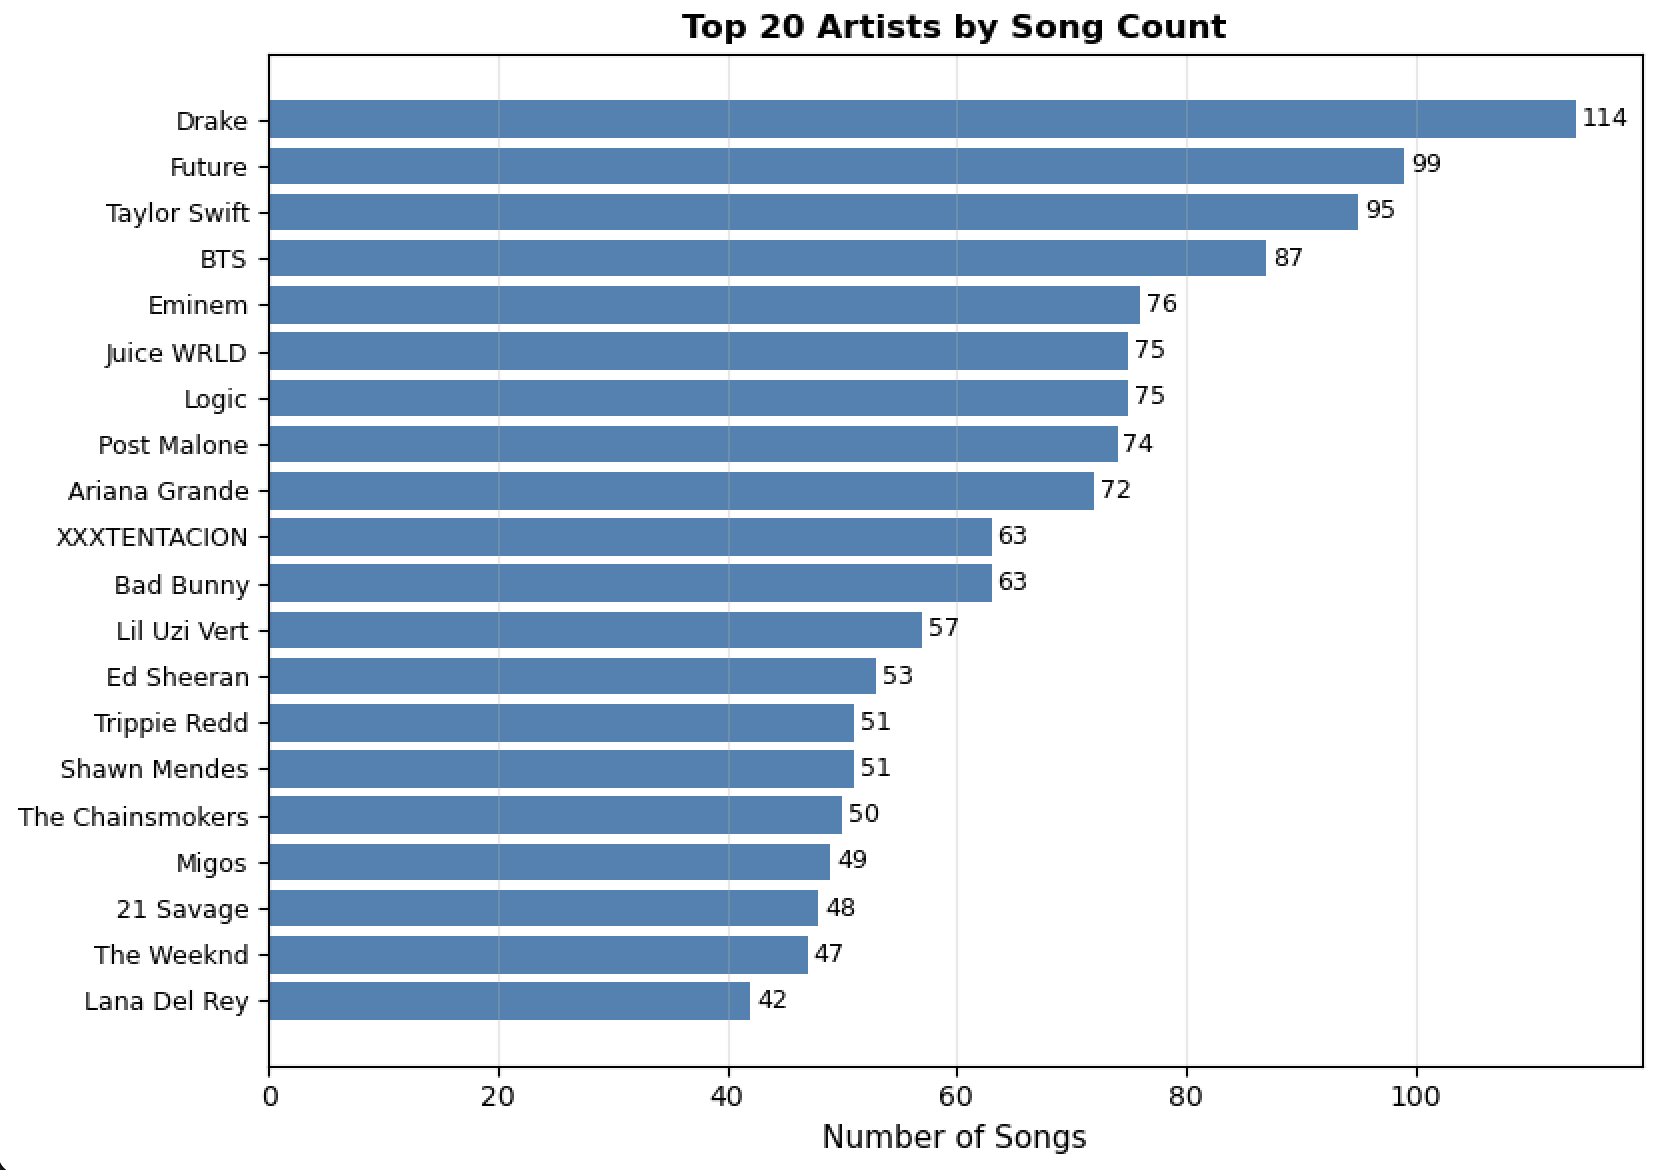
\includegraphics[width=\textwidth]{images/artist1.png}
    \caption{Top 20 Artists by Songs }
    \label{fig:artistsongcount}
\end{subfigure}
\begin{subfigure}{0.3\textwidth}
    \centering
    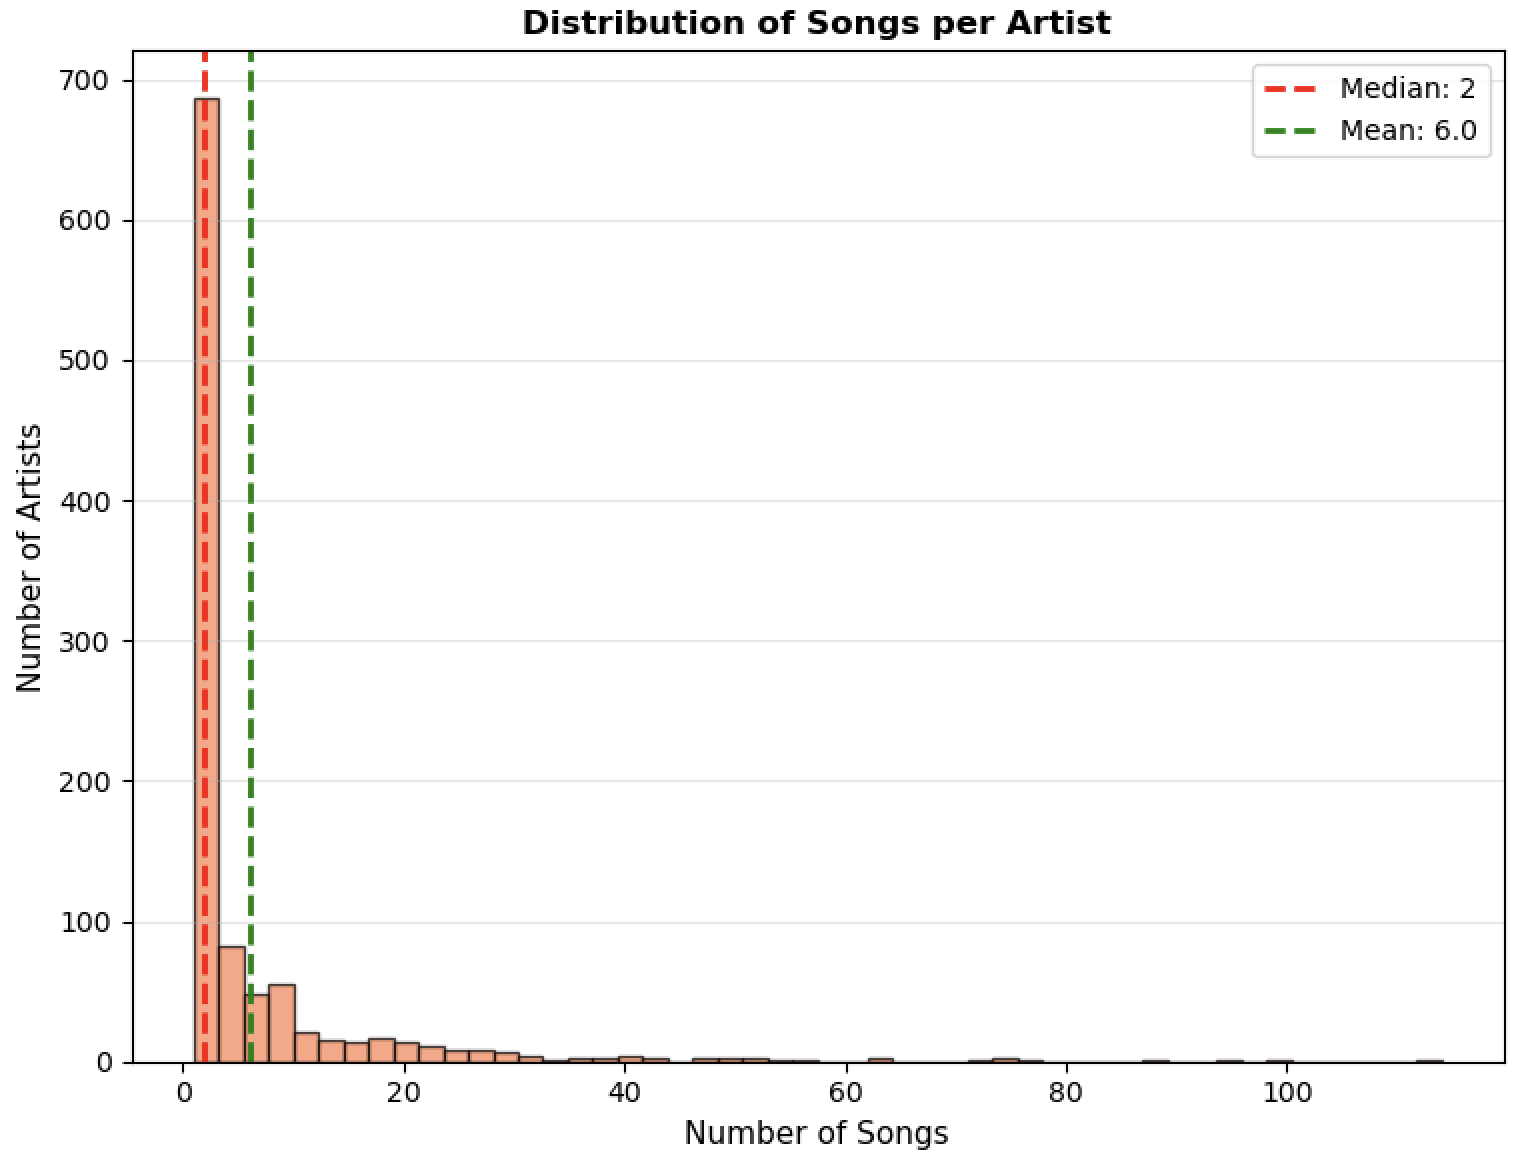
\includegraphics[width=\textwidth]{images/artist2.png}
    \caption{Distribution of Songs }
    \label{fig:songperartist}
\end{subfigure}

\caption{Top 20 Artists by Song count and Distribution of Songs per Artist}
\label{fig:two_plots}
\end{figure}
\vspace{-2em}
Figure 3(a) reveals that most songs (around 5,900 or 67\%) are released on Fridays, matching the industry practice of "New Music Friday" on streaming platforms. This Friday dominance also means more competition, which might affect chart success. Other days have much fewer releases (500-800 each), suggesting some artists avoid Fridays strategically. Figure 3(b) shows that most releases happen during regular months (7,600 songs) rather than the holiday season of November-December (1,600 songs, about 18\%). This suggests artists either avoid the competitive year-end period or strategically target holiday audiences and gift-buying seasons. Since release timing appears to affect chart performance, we included day of week and holiday season as features in our model. 

\vspace{-1em}
\begin{figure}[H]
\centering

\begin{subfigure}{0.3\textwidth}
    \centering
    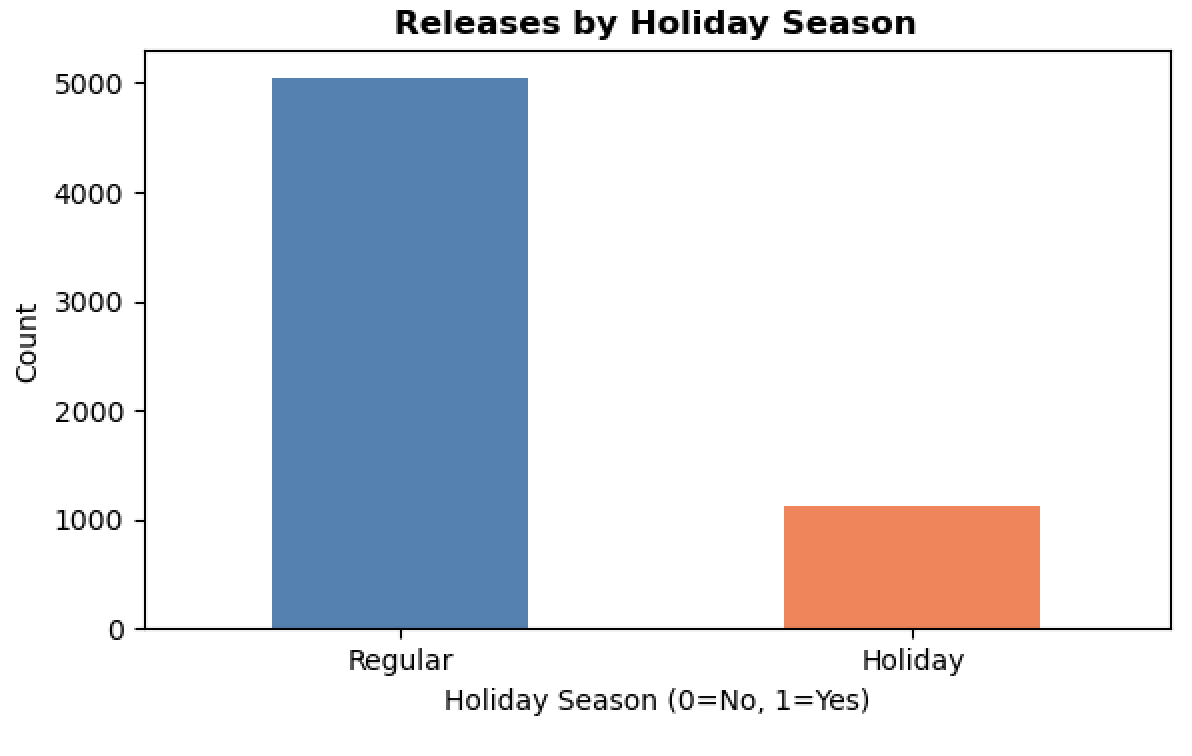
\includegraphics[width=\textwidth]{images/holiday.png}
    \caption{Releases by Holiday Season.}
    \label{fig:holiday}
\end{subfigure}
\begin{subfigure}{0.3\textwidth}
    \centering
    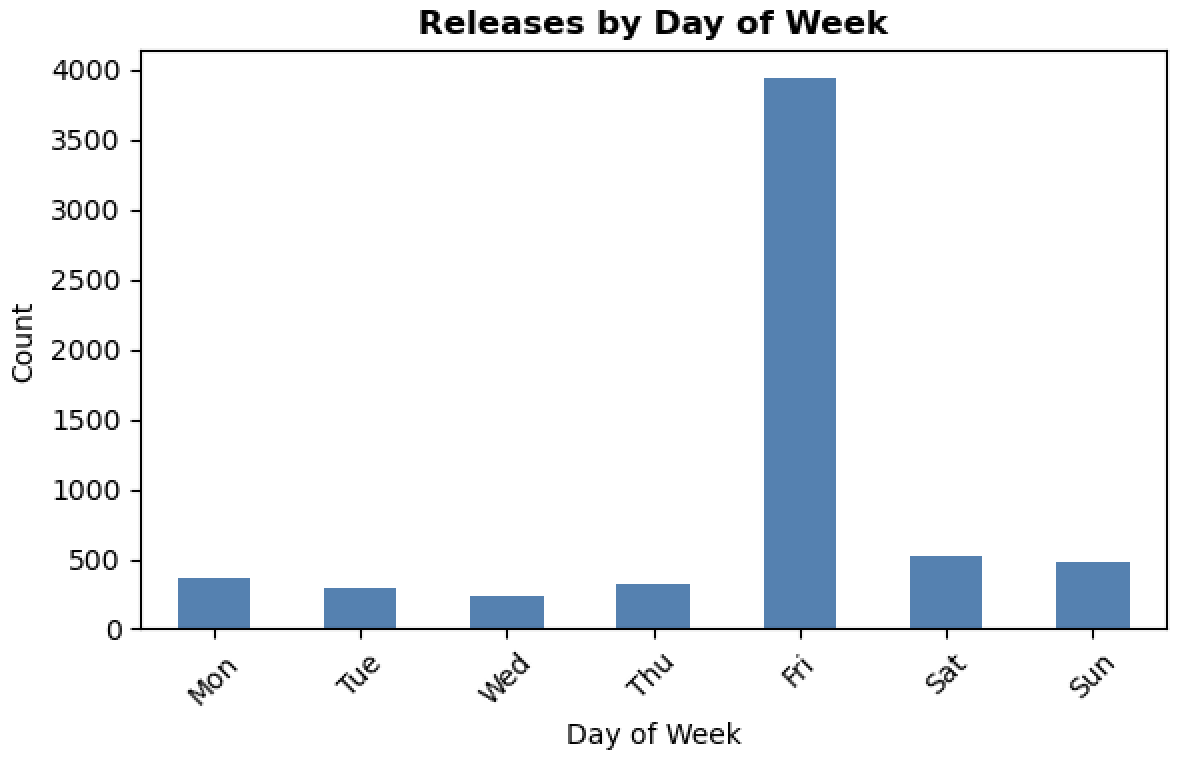
\includegraphics[width=\textwidth]{images/dayofweek.png}
    \caption{Releases by Day of the week.}
    \label{fig:dayofweek}
\end{subfigure}

\caption{Releases by Holiday Season and Releases by Day of Week}
\label{fig:two_plots}
\end{figure}
\vspace{-2em}


\section{Data preparation}
\subsection{Preprocessing}
Unlike standard classification tasks (e.g., email spam detection), the Spotify dataset is time-series data, meaning we cannot train on later years and evaluate on earlier years because key features such as artist popularity and chart rankings are time-dependent. To prevent data leakage from repeated or overlapping songs, we use a chronological 80/10/10 split for the training, validation, and test sets. The validation set is used for hyperparameter tuning and unbiased model selection, while 5-fold cross-validation is applied only on the training set to support hyperparameter tuning and hypothesis testing without violating the temporal structure of the data. We first use the raw training split to synthesis artist-level features, specifically artist popularity and collaboration. Artist features are computed from the training split and then applied to the validation and test sets. For the test set, artist features are derived from the combination of the training and validation splits. Next, the raw data for all three splits is aggregated to the song level, and temporal features are computed for each split. After generating all required features, each song-level dataset is assigned a popularity score (scaled from 0 to 100) using the equation described in \hyperref[eq:popularity_score]{Appendix B}. The popularity score is defined along two dimensions: peak score and longevity score\cite{ref6}. Longevity Score: the maximum weeks of song in chart. Peak Score: Measures the highest chart position achieved, calculated as the equation in \hyperref[eq:peak_score]{Appendix C}




The weighting coefficients were chosen to slightly favour longevity (0.60) over peak performance (0.4), reflecting the hypothesis that sustainable success is more indicative of genuine popularity than brief chart domination. After computing the popularity score across the dataset, songs are categorised by popularity, we have total 9161 songs for the model prediction. Songs with an overall popularity score above the 70th percentile are labelled as Popular, while those below this threshold are labelled as Not Popular. This percentile-based labelling strategy is widely used in academic research {\cite{PhamEtAl2015}. Finally, all engineered features are merged into the song-level dataset and standard scaled to ensure that all numeric features have a comparable scale. Standardisation prevents large-magnitude features from dominating model training and improves the stability of model learning. After labelling, the dataset contains approximately 30\% popular songs and 70\% non-popular songs across splits. Because the popular class is the minority, models tend to bias toward predicting the majority (non-popular) class, resulting in poor performance on the popular songs. To address this, we apply SMOTE (Synthetic Minority Over-sampling Technique) {\cite{smote}, which generates synthetic examples of the minority class through interpolation between existing samples rather than duplicating them. This technique produces a more balanced dataset, enables the model to learn clearer decision boundaries, and improves its ability to correctly identify minority-class instances without overfitting.

\subsection{Dimensionality Reduction}
Dimensionality reduction and feature extraction techniques are used on the training set as a preprocessing step. The reason behind such approaches is to reduce the complexity of the features fed into the model, resulting in reducing overfitting. However, our models have only 20 features considered as Baseline, which is not a significant number of ones. Therefore, dimensionality reduction may not provide substantial benefits. Nonetheless, we applied two methods that we consider suitable for our case. The first method is PCA, and the second is L1 regularisation {\cite{PhamEtAl2015}.

\noindent \textbf{Baseline} uses all available features, with a total of 20 features grouped as follows:First, the \textbf{audio features} include danceability, energy, loudness, speechiness, acousticness, instrumentalness, and valence. Second, the \textbf{temporal features} describe release time information, including release year, release quarter, release month, release day of week, is friday release, and is holiday season. Third, the \textbf{artist reputation features} capture the artist’s historical performance through artist song count, artist avg rank, and artist best rank. Finally, the \textbf{collaboration features} describe multi-artist interactions, including num collab artists, collab artist avg popularity, collab max frequency, and collab avg frequency.




\textbf{Principal Component Analysis (PCA)} is applied as a standard linear dimensionality reduction technique on the training set. Using the original 20 features, PCA reduces the feature space to 13 components, explaining 95\% of the total variance (as visualized in \hyperref[fig:PCA]{Appendix Q}


\textbf{L1 regularization} to force sparsity and identify the most discriminative predictors. By varying the inverse regularization strength ($C$), we observed that a value of $C=0.01$ yields an optimal balance between model complexity and performance \hyperref[fig:L1]{Appendix A}
. This configuration reduced the input space to ten significant features, achieving high accuracy while eliminating noise.  The ten features are selected namely  acoustic characteristics(Danceability, Loudness, Speechiness, Valence), temporal featrues( Release Week, Release Year, Friday Release), and artist popularity metrics (Average and Best Rank).



\section{Task 1: Popular song predict}

\subsection{Classification Algorithm}
We evaluated six classifiers to measure performance across variety levels of complexity. Logistic Regression and Linear SVM were established as linear baselines,while RBF SVM  assess non-linear decision boundaries.Also, we apply tree-based ensembles which are Random Forest, Gradient Boosting, and XGBoost leverage their inherent ability to capture high order feature interactions and robustness on structured tabular data.



\subsection{Metrics}
We use multiple metrics to evaluate our performance rather than relying solely on accuracy. Although accuracy provides an overall measure of correct predictions, it can be misleading in the presence of class imbalance. we also report the F1 score, which captures the harmonic mean of precision and recall for the Popular class and is more informative under imbalance. In addition, we consider The Area Under the Curve (AUC) of a Receiver Operating Characteristic (ROC), which measures discrimination capability across classification thresholds, and the confusion matrix, which provides a detailed breakdown of prediction Performance was evaluated on both training and test sets to assess potential overfitting. The test set metrics provide unbiased estimates of generalization performance. 

  

\subsection{Learning Method}
We divides the dataset into train, validation, and test sets following an 80/10/10 ratio. We evaluate six classification algorithms across three data representations, optimizing hyperparameters via GridSearchCV with 5-fold cross-validation on the training set. The validation set is then used for unbiased model selection. After tuning, we select the five best performing model base on their validation performance. These models are then evaluated on the test set using performance metric to provide an unbiased estimate of their generalisation ability. We also perform statistical hypothesis testing to determine whether the performance differences between models are statistically significant, which supports a more principled model selection process. Finally, we conduct a feature importance analysis to understand which features contribute most to the popular song predictions.  


\vspace{-1em}
\subsection{Results}
Evaluation of each optimised preprocessing classifier pair was conducted on the validation and test datasets to obtain Accuracy, F1, and ROC-AUC scores, with the top five models ranked by validation F1 listed in Table 1. For full representative data with models results are shown in 
\hyperref[fig:resultallrepresentation]{Appendix R}. Gradient Boosting with baseline features delivers strong validation accuracy and achieves the highest validation F1 score (Val Acc = 0.6301, Val F1 = 0.4545). We also find that the linear SVM consistently appears in the top-five rankings across all three feature representations (Baseline, PCA, and L1). Interestingly, XGBoost with baseline features exhibits the largest generalisation gap (Train Acc – Val Acc = 0.35), followed by Gradient Boosting with baseline features (0.29). Across the top-five models, performance consistently decreases from Train to Validation to Test sets, with all metrics showing the same downward trend. All models achieve validation ROC-AUC scores above 0.5, ranging from 0.58 to 0.69. Hyperparameter optimisation yielded a measurable improvement in classifier performance F1 +1.86\% ROC-AUC+12.39\%. The optimal hyperparameters identified for each model are provided in \hyperref[fig:Optimal_Hyper_parameter]{Appendix K}. 
The top ten features in the importance analysis from the model show that the highest-impact feature is artist average rank with a coefficient of –0.555, followed by artist best rank at –0.530. Loudness norm contributes positively with a coefficient of 0.317, while speechiness shows a strong negative effect at –0.307. Instrumentalness at –0.201, artist song count at –0.188, and acousticness at –0.169 follow next in importance. Holiday season contributes –0.124 and release day of week contributes 0.108. Valence has a smaller positive contribution at 0.081. Collaboration-related factors, including maximum collaboration frequency, average collaboration popularity, number of collaborating artists, and average collaboration frequency, each contribute –0.079. The least influential feature in this ranking is release year with a coefficient of –0.065 (Please see all the coefficient analysis in \hyperref[fig:Feature Importance]{Appendix I}.
\begin{table}[h!]
\centering
\caption{Complete Performance Metrics}

\resizebox{\textwidth}{!}{
\begin{tabular}{l c c c c c c c c c c c}
\toprule
\textbf{Feature Set + Model} &
\textbf{Train Acc} & \textbf{Val Acc} & \textbf{Test Acc} &
\textbf{Train F1} & \textbf{Val F1} & \textbf{Test F1} &
\textbf{Train ROC-AUC} & \textbf{Val ROC-AUC} & \textbf{Test ROC-AUC} &
\textbf{Gen. Gap} \\
\midrule

Baseline + Gradient Boosting &
0.9219 & 0.6301 & 0.5412 &
0.9217 & 0.4535 & 0.3231 &
0.9813 & 0.6492 & 0.4976 &
0.2918 \\

\textbf{Baseline + SVM (Linear)} &
\textbf{0.6160} & \textbf{0.4569} & \textbf{0.4216} &
\textbf{0.7158} & \textbf{0.4499} & \textbf{0.4303} &
\textbf{0.7187} & \textbf{0.5898} & \textbf{0.5310} &
\textbf{0.1591} \\

PCA + SVM (Linear) &
0.6296 & 0.4682 & 0.4399 &
0.7238 & 0.4462 & 0.4198 &
0.7230 & 0.5927 & 0.5324 &
0.1614 \\

Baseline + XGBoost &
0.9903 & 0.6358 & 0.5450 &
0.9902 & 0.4384 & 0.3081 &
0.9995 & 0.6550 & 0.4960 &
0.3545 \\

L1 + SVM (Linear) &
0.6672 & 0.5806 & 0.5853 &
0.7346 & 0.3955 & 0.3296 &
0.7345 & 0.5913 & 0.5248 &
0.0866 \\

\bottomrule
\end{tabular}
}
\end{table}
\vspace{-1em}
\subsection{Discussion}
The results show several key findings. First, XGBoost and Gradient Boosting both have large generalisation gaps, even though Gradient Boosting achieves high F1 and ROC-AUC on the validation set, indicating clear overfitting. In contrast, the linear SVM generalises well and appears in the top-five models across all three feature representations (Baseline, PCA, and L1). The PCA and L1 representations do not provide meaningful improvement over the baseline, which is consistent with our hypothesis test
\hyperref[tab:Hypothesis]{Appendix J} showing no significant difference. Across all five models, F1 performance remains low on both the validation and test sets, but all models achieve validation ROC-AUC above 0.5, meaning performance is still better than random. We select the Baseline with SVM (Linear) as the representative model because it has a small generalisation gap (Train Acc – Test Acc), and it provides the highest F1 score and ROC-AUC on the test set. And the representative features from baseline give us a better sense of interpret the results since L1 and PCA cut half of features to the model. From 20 features in feature-importance analysis shows that artist rankings are the most important features, suggesting that popular songs depend strongly on artist reputation rather than audio features alone. Among audio features, loudness has a positive coefficient, implying that louder songs tend to attract higher listener engagement, while speechiness and instrumentalness have negative coefficients, indicating that songs with more spoken content or long instrumental sections tend to be less popular. These findings differ from some academic works that report strong performance using audio features without artist representations{\cite{ref1}{\cite{ref2}{\cite{ref6}{\cite{PhamEtAl2015}. In our perspective, audio features appear less useful for predicting popularity unlike the other studies claimed. Note that our popularity score is constructed from chart rank and longevity, which may not fully reflect true popularity.


\section{Supplementary Task : Playlist suggestions based on listener mood}
\subsection{Unsupervised Algorithm}


Unsupervised learning techniques were employed to address the initial absence of explicit mood labels within the dataset. Specifically, the \textbf{K-Means clustering algorithm} was utilized to segment the data and identify inherent emotional groupings.

\subsection{Feature Selection and Clustering Parameters}

This process focused on the available musical attributes: \textbf{Energy} and \textbf{Valence} which served as the primary feature vectors for the clustering operation.

The segmentation strategy was directly informed by \textbf{Russel's Mood Classification Model} in \hyperref[fig:russel_model]{Appendix L}
\cite{russell1980circumplex}, which pre-determined the number of clusters to be four $K=4$  as \hyperref[fig:elbow]{Appendix M} 
This assignment ensured the resulting four clusters mapped directly to the model's four emotional quadrants, providing a theoretically grounded basis for mood classification.
\subsection{Clustering Algorithm }




Two clustering algorithms were applied: K-means, Gaussian Mixture Model (GMM) , the evaluation of these models using the calinski-harabasz index and david bouldin index provided quantitative measures of their performance 


\subsection{Evaluation Methodology and Result}

Several metrics were used to evaluate the performance of the clustering and prediction models, including:

\begin{tabular}{|l|p{6cm}|c|c|}
\hline
\textbf{Metric} & \textbf{Description} & \textbf{K-Means Score} & \textbf{GMM Score} \\
\hline
Silhouette Coefficient & Measures how similar an object is to its own cluster compared to other clusters (higher is better). & 0.3584 & 0.3158 \\
\hline
Calinski-Harabasz Index & Ratio of between-cluster dispersion to within-cluster dispersion (higher is better). & 7753.90 & 6877.33 \\
\hline
Davies-Bouldin Index & Measures the average similarity between clusters (lower is better). & 0.8881 & 1.0062 \\
\hline
\end{tabular}

Visual inspection of the clusters confirmed the distinct separation of data points, supporting the quantitative metrics. Consequently, K-Means was selected as the best-performing algorithm for clustering the data into different moods


\subsection{Discussion}
We can apply unsupervised learning to organize Spotify playlists. Clustering algorithms were performed on processed and standardized audio feature such as Energy and Valence from Spotify dataset. We decided to apply KMeans and Gaussian Mixture Model to measure their performance using silhouette score, Calinski-Harabasz Index, and Davies-Bouldin Index. KMeans is the best algorithm with the highest score in both KMeans and Calinski-Harabasz Index. However, considering only intrinsic metrics didn't show ideal results. We could not measure extrinsic measurement between our predicted labeled clustering and truth labeled. Also, due to the cut-off in the audio feature based on track id in Spotify API has been deprecated. We could not explore to do classification. This research lays the groundwork for future advancements in personalises music recommendation systems, aiming to enhance user satisfaction and engagement. 

\section{Conclusion}
Overall, the SVM (Linear) model provides the most reliable performance. Feature importance results indicate that artist reputation is the strongest predictor of popularity, while audio features contribute less. These findings differ from some academic studies that rely heavily on audio features, and our results suggest that such features alone are not sufficient. 
In suppliment task, evaluating the model using only intrinsic metrics did not yield ideal results, and we were unable to assess any extrinsic agreement between our predicted cluster labels and the true labels. In addition, our analysis was limited by the discontinuation of audio feature access via track IDs, as this functionality has been deprecated in the Spotify API.
\newpage


\bibliography{refs.bib}
\bibliographystyle{plain}
\newpage
\section*{Contribution}
s2810265
This member contributed to writing the Introduction, Exploratory Data Analysis, Preprocessin and Dimension reduction for representative, and Abstract sections of the report. They implemented the data preprocessing pipeline, feature synthesis for artist-level and collaboration features, conducted EDA, researched suitable classification methods, performed dimensionality reduction and feature selection, and carried out the post-hoc feature importance analysis.

s2777346
This member wrote the Task 1 Learning Methods, Results, Discussion, Conclusion, and Appendix sections. They reviewed the Task 1 codebase, assisted in data preprocessing, trained the classification models and tuned hyperparameters, and performed the evaluation of Task 1 models. Main coder and analyze Task 1

s2772327
This member wrote the Task 2 Learning Methods, Results, Discussion, and References sections. They researched clustering techniques, implemented clustering metrics for Task 2, trained and tuned the Task 2 models, and also reviewed part of the Task 1 and Supplement Task 2 code. Main coder and analyze for Task 2

s2845408
This member wrote the Task 2 section on Unsupervised Algorithms, feature selection explanation, and clustering parameter choices. They analysed clustering results by examining test-set metric performance, tested clustering configurations, and evaluated the Task 2 models. Also reviewed part of the Task 1 code.




\section*{Generative AI}
We used Generative AI to correct grammatical mistakes in our writing and improve the clarity of our project. Additionally, we used it to understand the IEEE citation format so that we could prepare our report in a proper and accurate manner. We also gathered key ideas to structure our paper effectively.

\newpage
\appendix
\section*{Appendice}
\section{L1 Feature Selection: Top 10 Most Important Features}


\vspace{2em}
\begin{figure}[H]
\centering
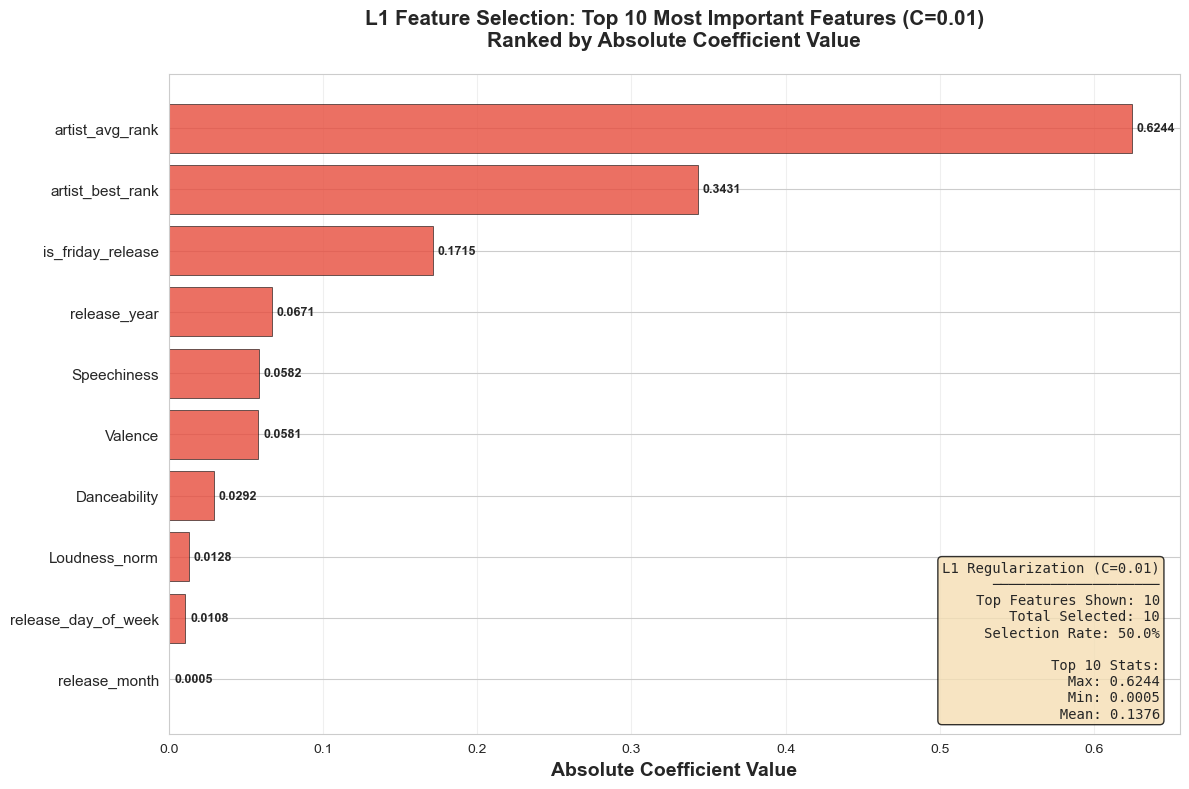
\includegraphics[width=0.6\linewidth]{images/L1 Features.png}
\caption{%
We apply L1 regularization to force sparsity and identify the most discriminative predictors. By varying the inverse regularization strength ($C$), we observed that a value of $C=0.01$ yields an optimal balance between model complexity and performance (Appendix X). This configuration reduced the input space to ten significant features, achieving high accuracy while eliminating noise. As shown in Figure X, the selected predictors encompass acoustic characteristics (e.g., Danceability, Loudness, Speechiness, Valence), temporal metadata (e.g., Release Year, Friday Release), and artist popularity metrics (Average and Best Rank).
}
\label{fig:L1}
\end{figure}
\vspace{2em}



\section{Popularity Score}

The popularity score is calculated as a weighted sum of peak position and chart duration, as shown in Equation \ref{eq:popularity_score}:

\begin{equation}
    \text{Popularity Score} = 0.40 \times \text{Peak Score} + 0.60 \times \text{Longevity Score}
    \label{eq:popularity_score}
\end{equation}

\noindent where the metrics are defined as follows
\begin{itemize}
    \item \textbf{Longevity Score:} The maximum number of weeks the song appeared in the chart.
    \item \textbf{Peak Score:} Measures the highest chart position achieved, calculated as $ \text{Peak Score} = \dots $ % Insert your formula here
\end{itemize}
\section{Peak Score}
\begin{equation}
    \text{Peak Score} = \frac{201 - \text{best\_rank}}{2} 
    \label{eq:peak_score}
\end{equation}

\noindent where \texttt{best\_rank} is the minimum rank value (closest to 1) achieved by the song.

Regarding the Popularity Score defined in Equation \ref{eq:popularity_score}, the weighting coefficients ($0.40$ and $0.60$) were chosen to slightly favor longevity over peak performance. This reflects the hypothesis that sustainable success is more indicative of genuine popularity than brief chart domination.
\newpage
\section{Audio Feature Specification}
\begin{table}[h]
\centering
\caption{Audio feature specifications}
\label{tab:Audio Feature} 
\begin{tabular}{p{3.5cm}p{2cm}p{6cm}}
\toprule
\textbf{Feature} & \textbf{Range} & \textbf{Description} \\
\midrule
Danceability & [0, 1] & Suitability for dancing based on tempo, rhythm stability, beat strength, and overall regularity \\
\midrule
Energy & [0, 1] & Perceptual measure of intensity and activity; high energy songs feel fast, loud, and noisy \\
\midrule
Loudness\_norm & [0, 1] & Overall loudness normalized from decibels; original range -34.475 to 1.509 dB \\
\midrule
Speechiness & [0, 1] & Presence of spoken words; values $>$ 0.66 indicate primarily speech, 0.33-0.66 indicate music with speech \\
\midrule
Acousticness & [0, 1] & Confidence measure that the track is acoustic (non-electronic) \\
\midrule
Instrumentalness & [0, 1] & Predicts whether a track contains no vocals; values $>$ 0.5 indicate instrumental tracks \\
\midrule
Valence & [0, 1] & Musical positiveness; high valence sounds positive/cheerful, low valence sounds sad/angry \\
\bottomrule
\end{tabular}
\end{table}

\section{Hyperparameter grids used for model selection}

\begin{table}[h!]
\centering
\caption{Hyperparameter grids used for model selection}
\label{tab:HyperGrids} 
\setlength{\tabcolsep}{6pt}
\renewcommand{\arraystretch}{1.25}

\begin{tabular}{p{0.22\textwidth} p{0.33\textwidth} p{0.33\textwidth}}
\toprule
\textbf{Classifier} & \multicolumn{2}{c}{\textbf{Parameters [Options]}} \\
\midrule

Logistic Regression &
$C$ [0.05, 0.1, 1, 5, 10] &
Solver [lbfgs, liblinear] \\

SVM (Linear) &
$C$ [0.1, 1, 10] &
-- \\

SVM (RBF) &
$C$ [0.1, 1, 10] &
$\gamma$ [scale, 0.01, 0.1] \\

Random Forest &
$n_{\text{estimators}}$ [10, 20, 50, 100, 200, 400] &
Max depth [None, 10, 20] \\
&
Min samples split [2, 5] &
Min samples leaf [1, 2];    Max features [sqrt, log2] \\

Gradient Boosting &
$n_{\text{estimators}}$ [10, 20, 50, 100, 200] &
Learning rate [0.05, 0.1, 0.2]; Max depth [2, 3, 4] \\

XGBoost &
$n_{\text{estimators}}$ [10, 20, 50, 100, 200, 400] &
Max depth [4, 6, 8] \\
&
Learning rate [0.05, 0.1, 0.2] &
Subsample [0.7, 0.9, 1.0]; Colsample\_bytree [0.7, 0.9, 1.0] \\
&
$\lambda$ (reg\_lambda) [0.5, 1.0, 2.0] &
$\alpha$ (reg\_alpha) [0, 0.1, 0.5] \\

\bottomrule
\end{tabular}
\end{table}

\newpage

\renewcommand{\thesubsection}{\thesection.\arabic{subsection}}

\newpage




\section{Metrics Purpose and Features}

\begin{tabular}{|p{4.5cm}|p{8.5cm}|}
\hline
\textbf{Clustering Algorithm} & \textbf{Purpose and Features} \\
\hline
\textbf{K-Means} & Simplicity, scalability to large datasets, and a convergence guarantee. Minimizes the distance between each data point and its assigned cluster centroid (within-cluster sum of squares). \\

\hline
\textbf{Gaussian Mixture Model (GMM Clustering)} & Models data points with a mixture of Gaussian (Normal) distributions. Provides probabilistic cluster assignments. **Does not require the number of clusters ($K$) to be specified beforehand** (though $K$ is often a hyperparameter). Can model clusters with non-spherical shapes (ellipsoidal). \\
\hline
\end{tabular}

\section{Classification Report for Random Forest (Final Model)}

\begin{table}[h!]

\centering
\caption{Classification Report for Random Forest (Final Model)}

\begin{tabular}{lcccc}

\toprule

\textbf{Class} & \textbf{Precision} & \textbf{Recall} & \textbf{F1-Score} & \textbf{Support} \\

\midrule

Anxiety       & 0.97 & 0.96 & 0.97 & 23790 \\

Contentment   & 0.96 & 0.96 & 0.96 & 13982 \\

Depression    & 0.96 & 0.97 & 0.97 & 29997 \\

Exuberance    & 0.95 & 0.95 & 0.95 & 25644 \\

\midrule

\textbf{Accuracy}     & \multicolumn{3}{c}{0.96} & 93413 \\

\textbf{Macro Avg}    & 0.96 & 0.96 & 0.96 & 93413 \\

\textbf{Weighted Avg} & 0.96 & 0.96 & 0.96 & 93413 \\

\bottomrule

\end{tabular}

\end{table}
\section{Cluster plot comparison of K-means (left) and GMM (right)}

\begin{figure}[H]
    \centering
    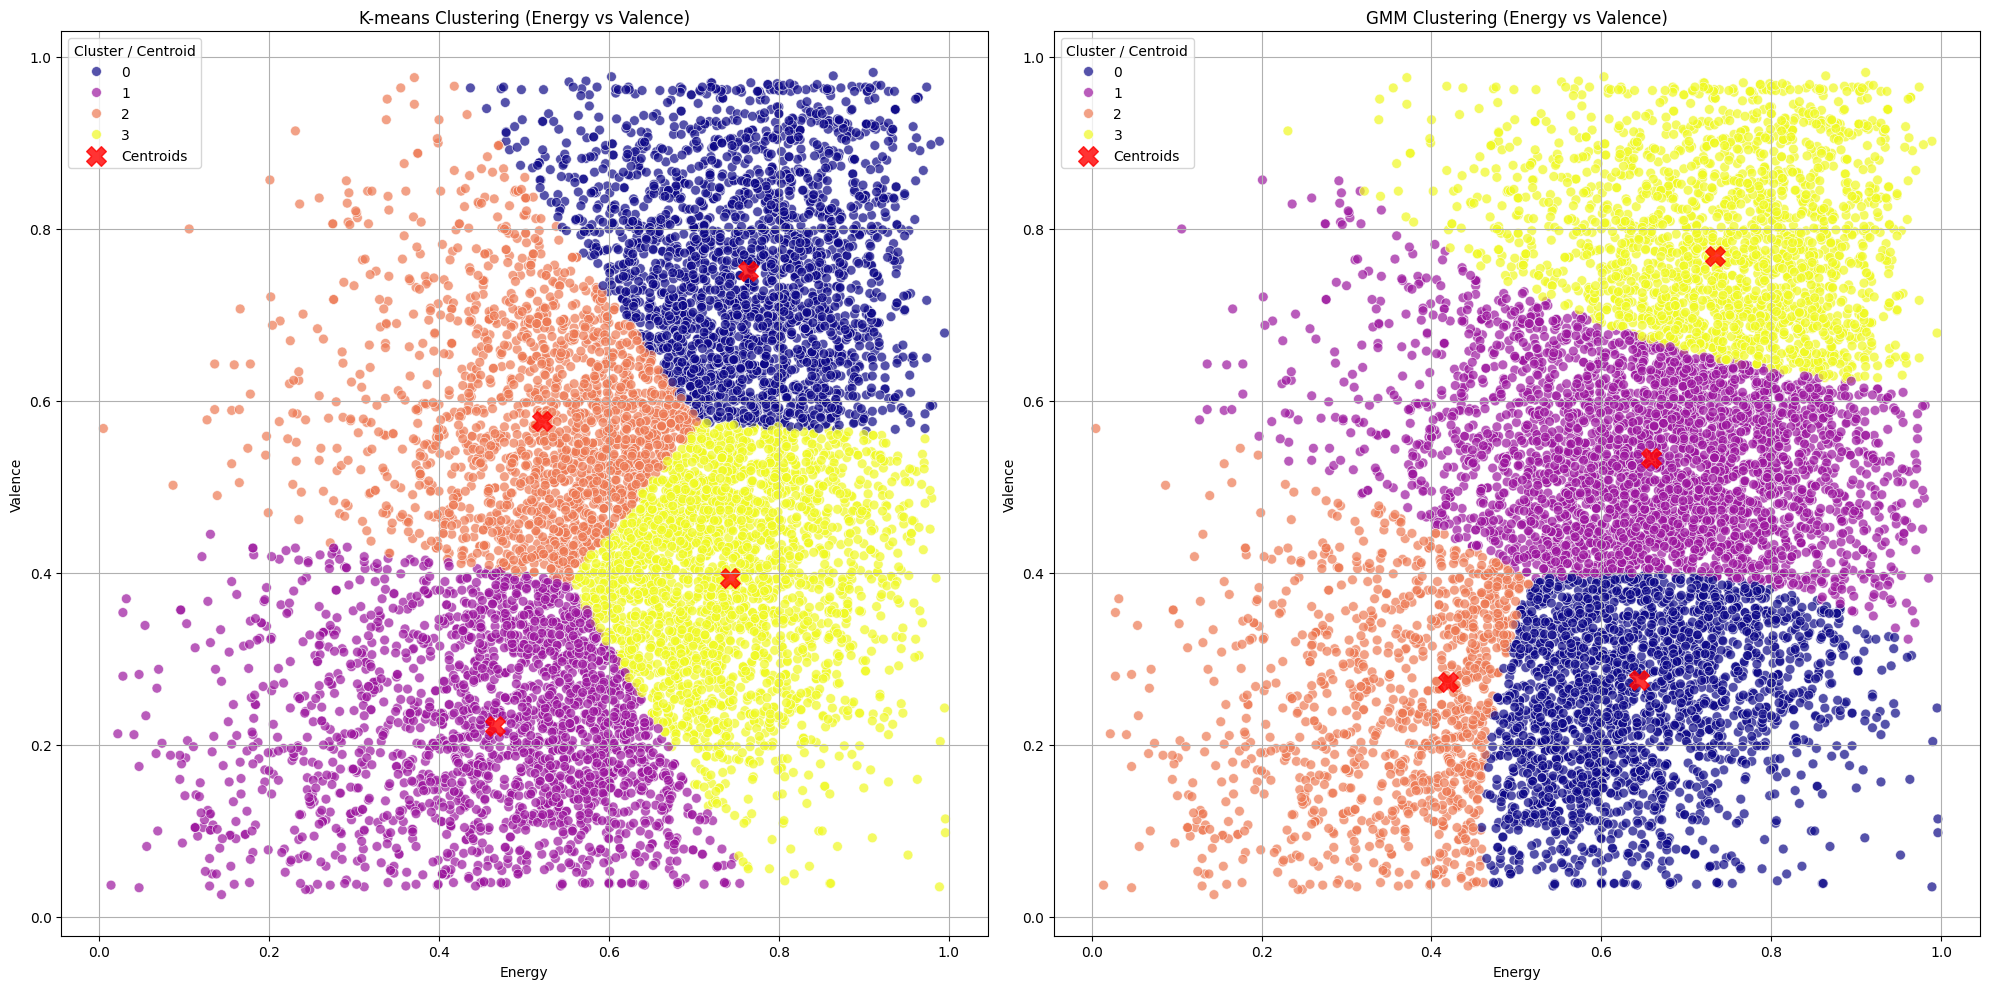
\includegraphics[width=0.6\linewidth]{images/clustering.png}
    \caption{Cluster plot comparison of K-means (left) and GMM (right).}
    \label{fig:appendix_clustering} % <--- Note the new label
\end{figure}
 

\section{Feature Importance Analysis}

\begin{figure}[H]
    \centering
    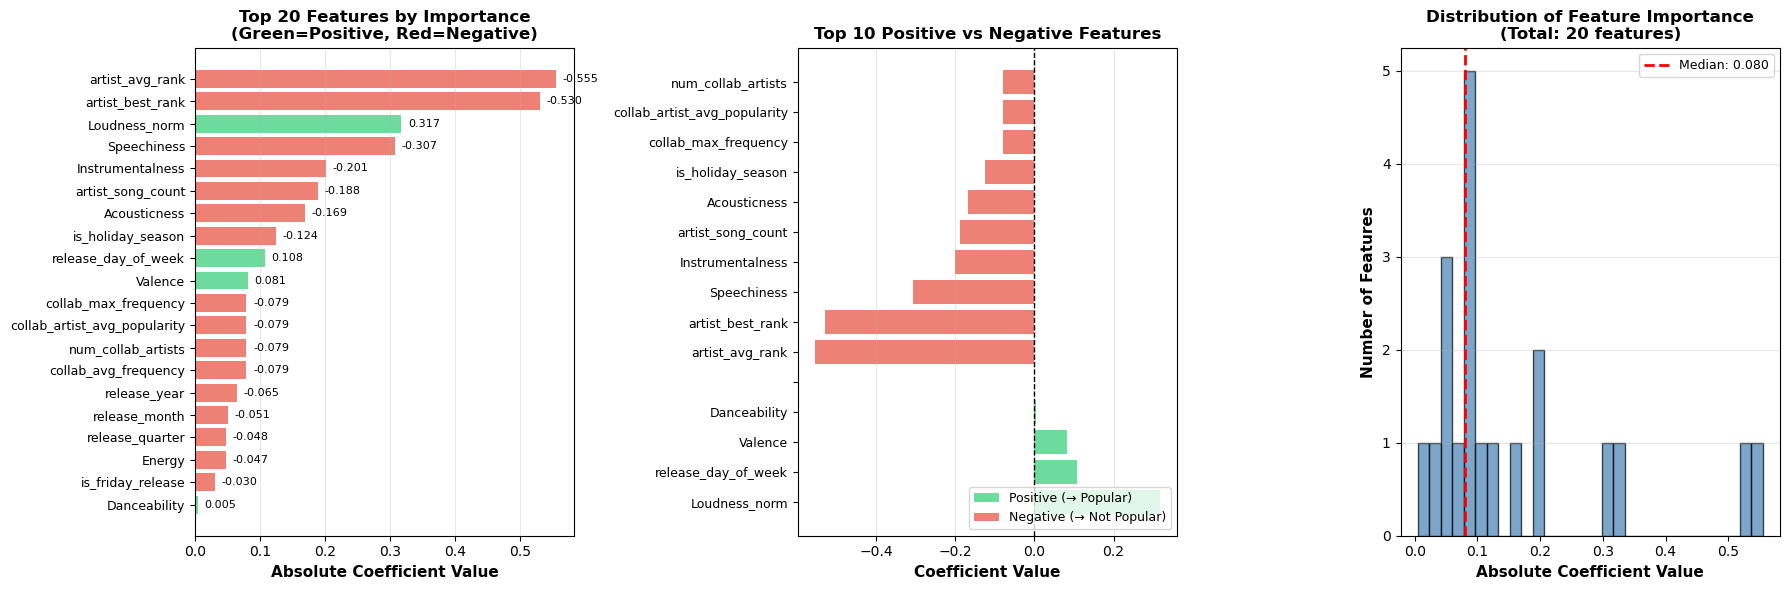
\includegraphics[width=\linewidth]{images/FeatureImportance.png}
    \caption{Feature Importance Analysis}
    \label{fig:Feature Importance} % <--- Note the new label
\end{figure}


\section{Hypothesis test}


\begin{quote}
\label{tab:Hypothesis}
\ttfamily
Test 1: SVM Baseline vs SVM + L1\\
Baseline: 0.7287 ± 0.0084\\
L1: 0.7201 ± 0.0056\\
t-statistic: 1.617\\
p-value: 0.1813\\
No significant difference (p $\ge$ 0.05)\\

Test 2: SVM Baseline vs SVM + PCA\\
Baseline: 0.7287 ± 0.0084\\
PCA: 0.7257 ± 0.0114\\
t-statistic: 0.800\\
p-value: 0.4683\\
No significant difference (p $\ge$ 0.05)\\

Test 3: SVM + L1 vs SVM + PCA\\
L1: 0.7201 ± 0.0056\\
PCA: 0.7257 ± 0.0114\\
t-statistic: -0.987\\
p-value: 0.3793\\
No significant difference (p $\ge$ 0.05)\\

\textbf{VERIFICATION ON HELD-OUT VALIDATION SET}\\
SVM Baseline: Val F1 = 0.4499, Val Acc = 0.4569\\
SVM + L1: Val F1 = 0.3955, Val Acc = 0.5806\\
SVM + PCA: Val F1 = 0.4462, Val Acc = 0.4682
\end{quote}

\section{Optimal Hyper-parameter}

\begin{figure}[H]
    \centering
    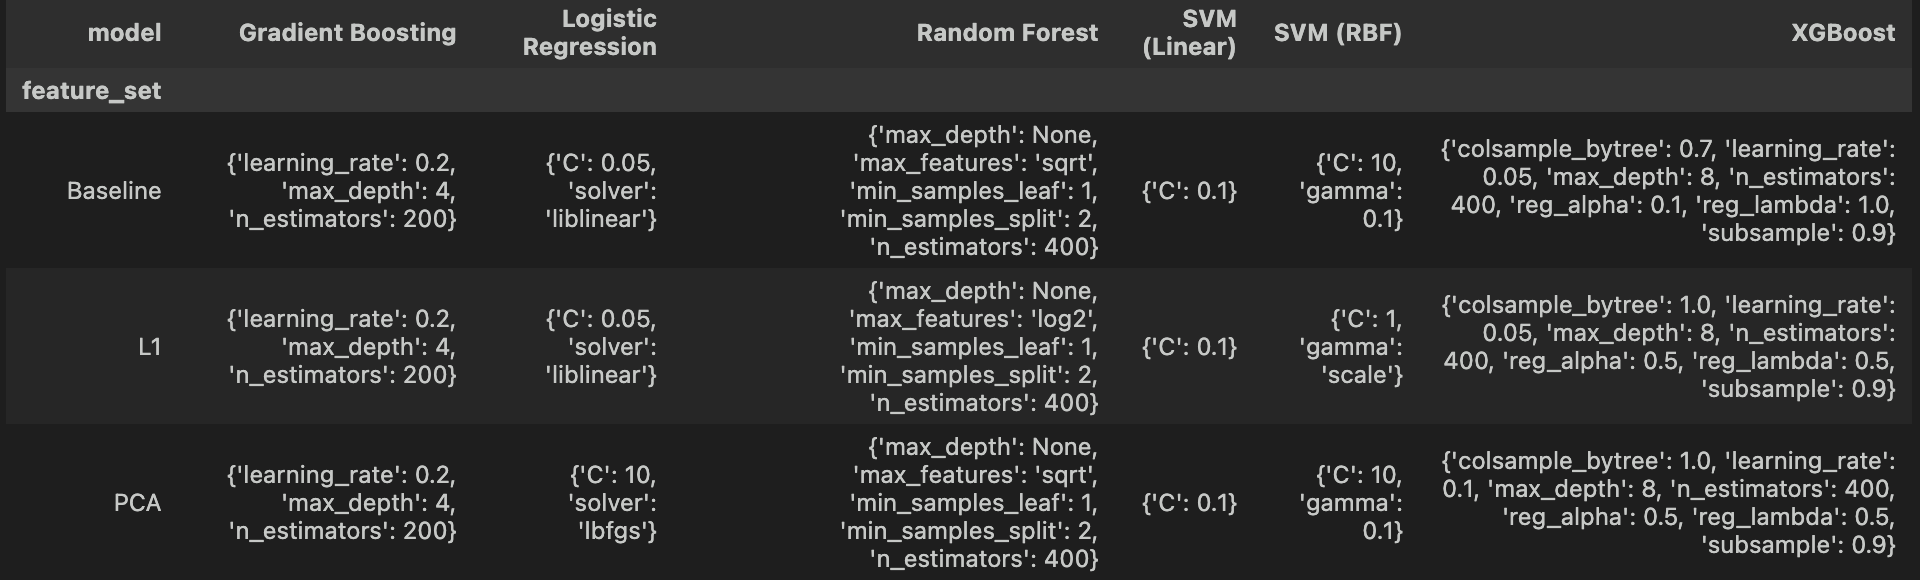
\includegraphics[width=\linewidth]{images/optimal parameter.png}
    \caption{Optimal Hyper-parameter}
    \label{fig:Optimal_Hyper_parameter} % <--- Note the new label
\end{figure}


\section{Russel}

\begin{figure}[H]
    \centering
    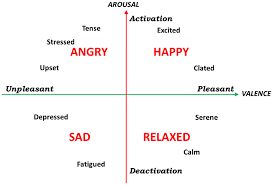
\includegraphics[width=\linewidth]{images/russel.png}
    \caption{Russel Model}
    \label{fig:russel_model} % <--- Note the new label
\end{figure}

\section{Elbow Technique}
\begin{figure}[H]
    \centering
    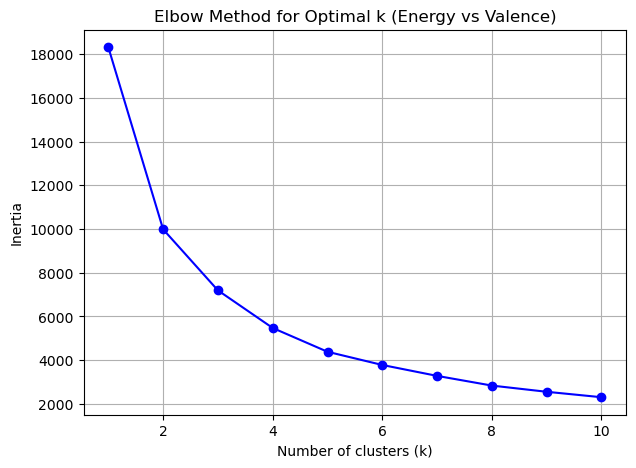
\includegraphics[width=\linewidth]{images/elbow.png}
    \caption{Elbow Technique  K-Means}
    \label{fig:elbow} % <--- Note the new label
\end{figure}


\section{Temporal Features}

Temporal features capture release timing patterns, calculated from the \texttt{first\_appearance} date for all splits.

\begin{table}[htbp]
\centering
\caption{Temporal feature specifications}
\label{tab:temporal_features}
\begin{tabular}{lll}
\toprule
\textbf{Feature} & \textbf{Range} & \textbf{Description} \\
\midrule
release\_year & [2017, 2023] & Year of song release extracted from \\
& & first appearance date \\
\addlinespace
release\_quarter & [1, 4] & Quarter of release (Q1=Jan-Mar, Q2=Apr-Jun, \\
& & Q3=Jul-Sep, Q4=Oct-Dec) \\
\addlinespace
release\_month & [1, 12] & Month of release (1=January, 12=December) \\
\addlinespace
release\_day\_of\_week & [0, 6] & Day of week for release (0=Monday, \\
& & 6=Sunday); captures industry release patterns \\
\addlinespace
is\_friday\_release & \{0, 1\} & Binary indicator if song released on Friday; \\
& & 1=Friday release, 0=other day \\
\addlinespace
is\_holiday\_season & \{0, 1\} & Binary indicator if released in November or \\
& & December; 1=holiday season, 0=other months \\
\bottomrule
\end{tabular}
\end{table}


\section{Artist Features}

Artist features capture historical performance and reputation, calculated from training period data (2017-2021) only. For new artists not in training data, default values are shown in parentheses.

\begin{table}[htbp]
\centering
\caption{Artist feature specifications}
\label{tab:artist_features}
\begin{tabular}{lll}
\toprule
\textbf{Feature} & \textbf{Range} & \textbf{Description} \\
\midrule
artist\_song\_count & [1, 114] & Number of unique songs by artist that \\
& & charted in training data (default: 1) \\
\addlinespace
artist\_avg\_rank & [31.02, 200] & Average rank across all chart appearances \\
& & in training data; lower is better (default: 134.78) \\
\addlinespace
artist\_best\_rank & [1, 200] & Best (lowest) rank achieved by artist \\
& & across all songs in training data (default: 71.50) \\
\bottomrule
\end{tabular}
\end{table}

\section{Artist Features}

Artist features capture historical performance and reputation, calculated from training period data (2017-2021) only. For new artists not in training data, default values are shown in parentheses.

\begin{table}[htbp]
\centering
\caption{Artist feature specifications}
\label{tab:artist_features}
\begin{tabular}{lll}
\toprule
\textbf{Feature} & \textbf{Range} & \textbf{Description} \\
\midrule
artist\_song\_count & [1, 114] & Number of unique songs by artist that \\
& & charted in training data (default: 1) \\
\addlinespace
artist\_avg\_rank & [31.02, 200] & Average rank across all chart appearances \\
& & in training data; lower is better (default: 134.78) \\
\addlinespace
artist\_best\_rank & [1, 200] & Best (lowest) rank achieved by artist \\
& & across all songs in training data (default: 71.50) \\
\bottomrule
\end{tabular}
\end{table}

\section{PCA}


\begin{figure}[H]
    \centering
    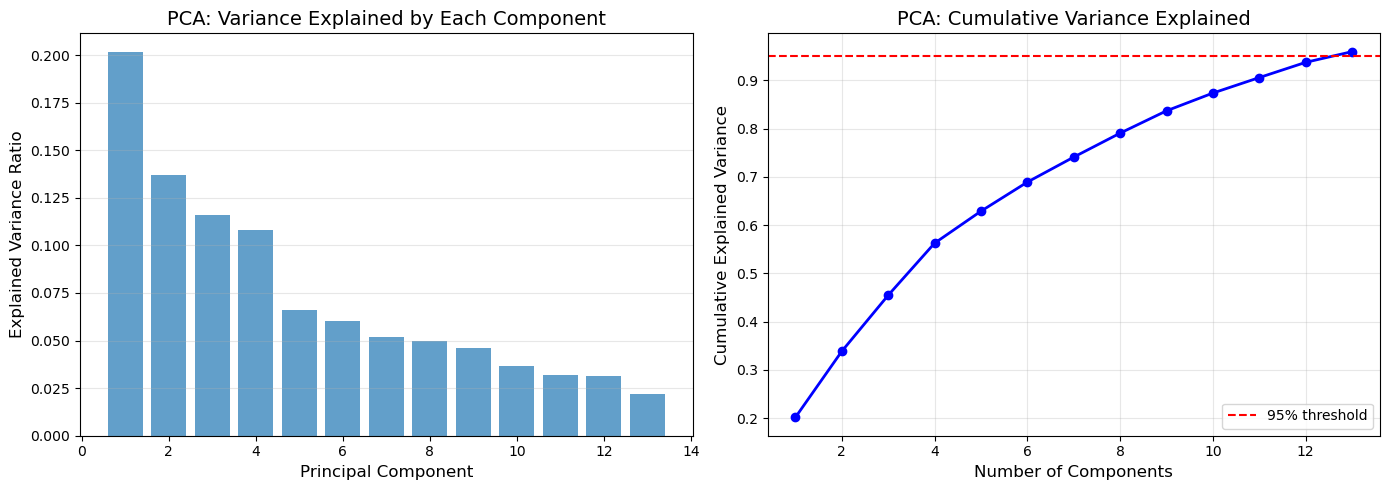
\includegraphics[width=\linewidth]{images/PCA.png}
    \caption{Feature Importance Analysis}
    \label{fig:PCA} % <--- Note the new label
\end{figure}

\section{ All matric evaluation from learning model for all representation and models}

\begin{figure}[H]
    \centering
    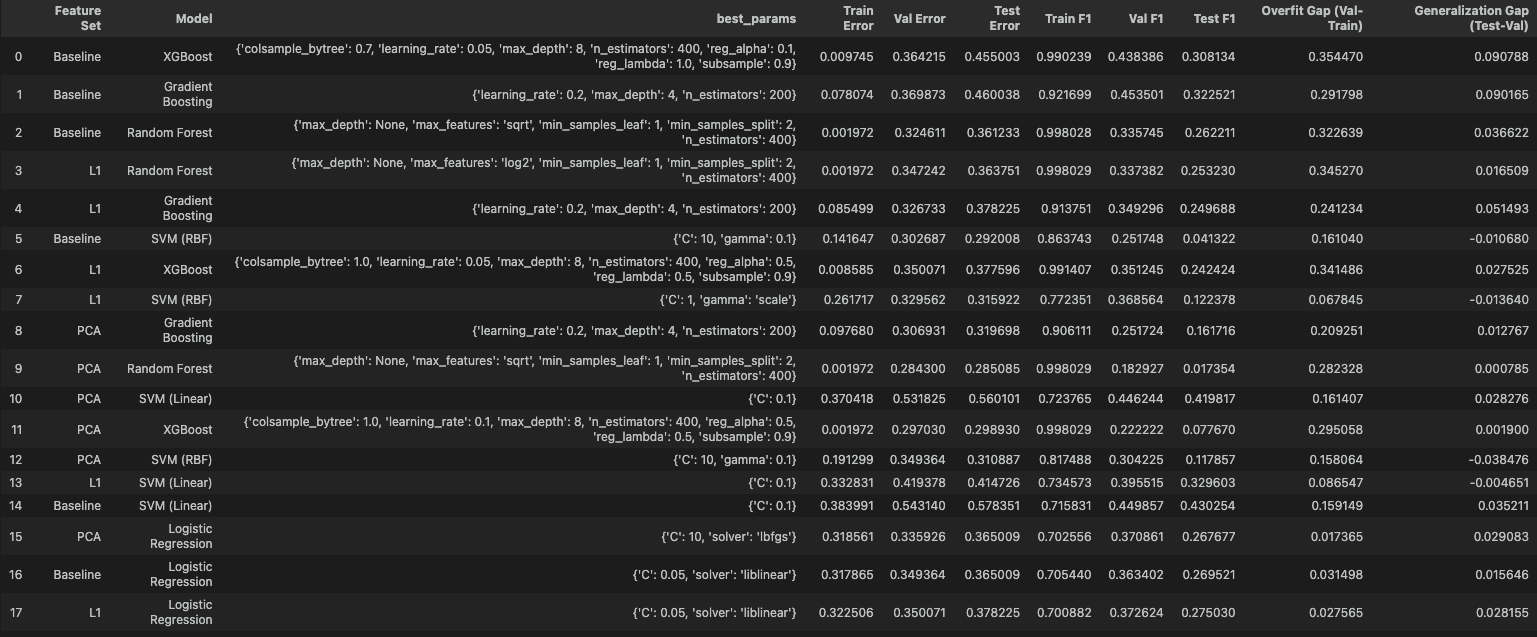
\includegraphics[width=1.0\linewidth]{images/allresult.png}
    \caption{ All results for all representation}
    \label{fig:resultallrepresentation} % <--- Note the new label
\end{figure}


\end{document}







%%% Local Variables:
%%% mode: latex
%%% TeX-master: t
%%% End:

